\chapter{Planejamento das Avaliações}

\section{Divisão das metas nas iterações}
\begin{figure}[h!]
  \centering
    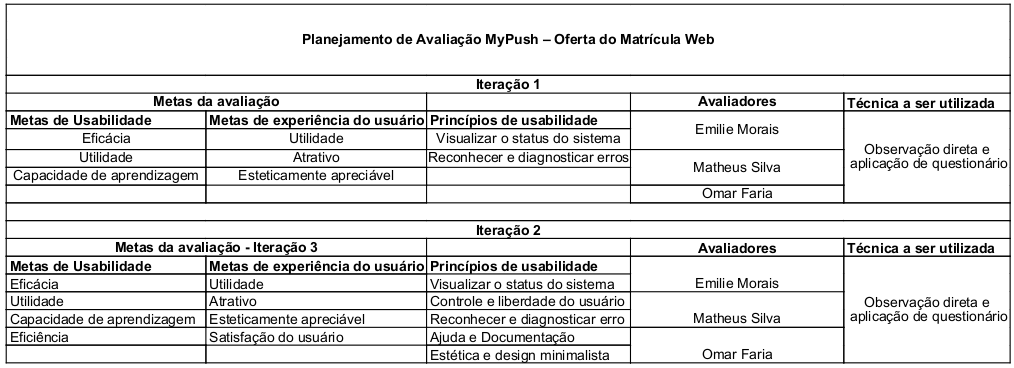
\includegraphics[keepaspectratio=true, scale=0.5]{figuras/planejamentoavaliacoes.png}
  \caption{Planejamento das avaliações}
  \label{Planejamento}
\end{figure}

% \begin{figure}[h!]
%   \centering
%     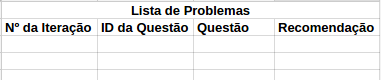
\includegraphics[keepaspectratio=true, scale=0.7]{figuras/listaproblemas.png}
%   \caption{Lista de problemas a ser preenchida nas avaliações}
% \end{figure}
% 

\section{Relatório Consolidado}

O modelo de relatório Consolidado pode ser visto no Apêndice D, no qual encontram-se três modelos,
um para avaliações do protótipo de papel, um para avaliações do protótipo da ferramenta e um para avaliação de acessibilidade. Nesse relatório
são sumarizados os resultados qualitativos e os quantitativos. Esses resultados foram divididos em métodos
de avaliação sugeridos por \cite{BARBOSA}

\subsection{Resultados qualitativos}

\subsubsection{Método de investigação}
Através de uma rápida entrevista com o usuário serão obtidas algumas informações além do questionário.

\subsubsection{Problemas encontrados nas avaliações}

Se o usuário durante ou depois da avaliação relatar algum problema, o mesmo deve ser registrado na tabela abaixo.
\begin{table*}[!h]
\caption{Lista de problemas a ser preenchida nas avaliações. Fonte: \cite{preece} adaptado}
\label{tab:problema}
  \begin{tabular}{p{0.18\linewidth}p{0.18\linewidth}p{0.30\linewidth}p{0.30\linewidth}}
  \hline
    Nº da Iteração & ID da Questão & Questão & Recomendação\\
 \hline
  \end{tabular}
\end{table*}

\subsection{Resultados quantitativos}

  \subsubsection{Método de investigação}
  Cada questão dos questionário será avaliada de 0 a 5 e assim serão obtidos resultados numéricos
  em relação a cada meta a ser avaliada.

  
  \subsubsection{Método de inspeção}
  Esse método será aplicado na versão \textit{Desktop} do protótipo de modo a avaliar a acessibilidade da página.
  Essa avaliação será realizada através da ferramenta ASES e \textit{Colour Contrast Analyser} e também será
  verificado a aderência a alguns itens do \textit{checklist} do desenvolvedor contido no eMAG \cite{emag}.
  
  Os itens a serem verificados estão na tabela \ref{tab:emag}.
  
  \begin{table*}[!h]
\caption{Itens do eMAG. Fonte: \cite{emag} adaptado}
\centering
\label{tab:emag}
  \begin{tabular}{p{0.40\linewidth}p{0.40\linewidth}}
  \hline
  O site fornece a localização do usuário em um conjunto de páginas? & Você está em: Página inicial > Downloads\\
  \hline
  Há um campo de busca no site? O resultado da busca é de fácil acesso? & No caso de sites extensos é importante o uso de um campo de busca. Esse campo, quando utilizado, deve remeter o seu foco no início do resultado da busca.\\
\hline
% Os menus estão em forma de lista? Quando há submenus ocultos, é disponibilizado um aviso para mostrar/ocultar esses sub­menus? & Os menus devem estar em forma de lista/itens.  \\
% \hline
Existe o Mapa do Site? & Para melhorar a navegação o site deve conter uma página com o Mapa do Site O mapa deve ser apresentado, de preferência, em forma de lista, assim como um sumário, e deve conter os principais links de conteúdos. Sugerimos utilizar tantos níveis quantos forem necessários\\
 \hline
  \end{tabular}
\end{table*}

  
  \subsubsection{Método de observação}
  Serão obtidos valores numéricos para algumas metas utilizando-se de métricas de qualidade obtidas na
  norma \citeonline{iso}.
  
\vfill
\pagebreak
\subsubsubsection{Métricas a serem utilizadas nas avaliações}
\begin{figure}[!h]
  \centering
    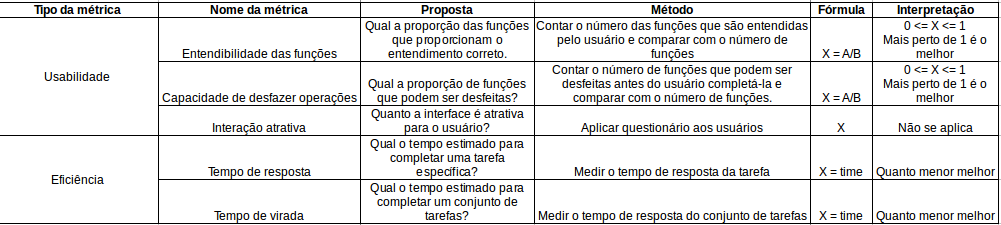
\includegraphics[keepaspectratio=true, scale=0.6, angle=-90]{figuras/qualidade.png}
  \caption{Métricas de Qualidade. Fonte: \cite{iso}}
  \label{fig:metricas}
\end{figure}

\pagebreak

% \section{Iteração 1}
% 
% \begin{figure}[h!]
%   \centering
%     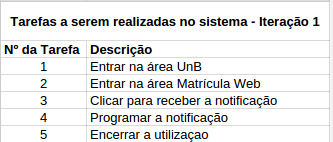
\includegraphics[keepaspectratio=true, scale=0.7]{figuras/tarefas1.png}
%   \caption{Lista de Tarefas para os usuários na Iteração 1}
% \end{figure}
% 
% \begin{table*}[!h]
% \caption{Lista de problemas. Fonte: \cite{preece} adaptado}
% \label{Rotulo}
%   \begin{tabular}{p{0.18\linewidth}p{0.18\linewidth}p{0.30\linewidth}p{0.30\linewidth}}
%   \hline
%     Nº da Iteração & ID da Questão & Questão & Recomendação\\
%  \hline
%   \end{tabular}
% \end{table*}